\documentclass{standalone}
\usepackage{standalone}

\begin{document}
\subsection{Rescale}
By minimizing the size of an image we can reduce processing time dramatically. But reducing image may result in loss of information. From reviews, we decided to use the dimension: $640 \times 480$. We re-scale the input image into this dimension at first step. Figure \ref{fig:RescaledSample} shows a sample image.
\begin{figure} 
	\centering
	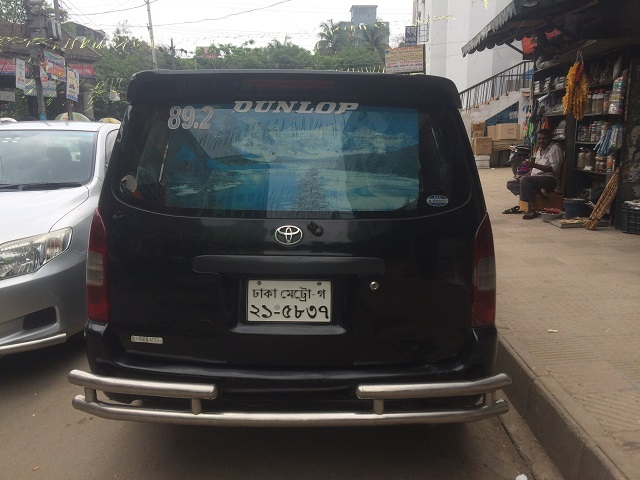
\includegraphics[width=.8\linewidth]{./img/sample/stage0.jpg}
	\caption{A sample input image (rescaled)}
	\label{fig:RescaledSample}
\end{figure}

\end{document}